\documentclass[a4paper,11pt]{report}
\usepackage[utf8x]{inputenc}
\usepackage[pdftex]{graphicx}
\usepackage[cm]{fullpage}
\usepackage{subfig}
\usepackage{url}
%\usepackage{showkeys}
\usepackage{gensymb}

\renewcommand{\topfraction}{.9}
\renewcommand{\bottomfraction}{.9}
\renewcommand{\textfraction}{.1}

\title{Performance Evaluation of a UAV-mounted LIDAR and camera for Traversability Assessment - Preliminary Report}
\author{Paul D. Cox, Intern at LAAS-CNRS, 5AE INSA Toulouse}

\begin{document}
\maketitle

\tableofcontents
\newpage

\chapter{Project Background and Motivation}

\section{Report Purpose}

This report's purpose is to present the ideas behind this project and the progress so far. It also includes practical discussions intended to guide the group as it attempts to broaden its use of UAVs. A literature review has been significantly delayed due to the early technical advancement necessary to adequately plan for the June competition, rendering a theoretical analysis at this stage impossible. The author hopes that a more than cursory review of the field and how this project fits into it can be presented in the final report.

\section{LAAS Robotics}

The Robotics and Interactions (RIS) group of the LAAS operates a number of robots that serve as testbeds for algorithm development and research \cite{ugvs}. These indoor and outdoor robots are primarily UGVs adapted for various tasks or needs. For example, Rackham (Figure \ref{fig:Rackham}) is equipped with a plethora of vision and proximity sensors \cite{rackham}, while Jido (Figure \ref{fig:Jido}) is outfit with a manipulator \cite{jido}, and Dala (Figure \ref{fig:Dala}) is capable of high-speed outdoor travel \cite{dala}. The group is interested in complementing its ground-based fleet with airborne vehicles. The intent is to research cooperative scenarios where the airborne vehicles provide a sensing advantage due to their unique perspective and mobility. More specifically, the group decided to include a UAV in this years ELROB competition attempt, and this project will be to create that UAV \cite{this}. 

\begin{figure}[htb]
  \centering
  \subfloat[Rackham]{\label{fig:Rackham}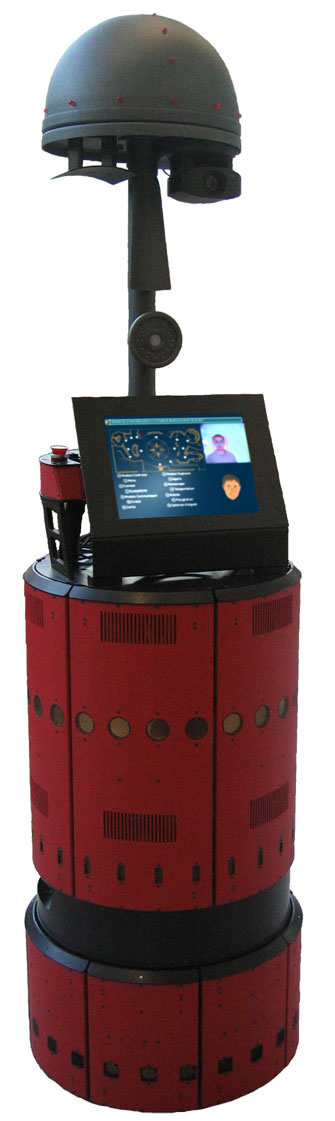
\includegraphics[width=25mm]{rackham.png}}                
  \subfloat[Jido]{\label{fig:Jido}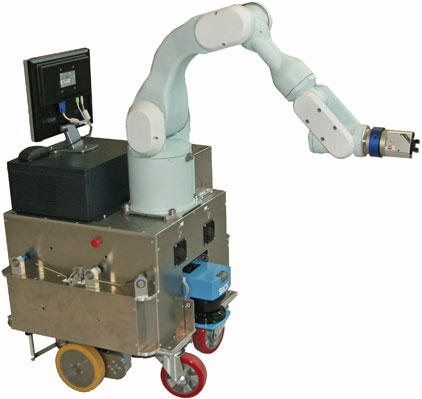
\includegraphics[width=40mm]{jido.png}}
  \subfloat[Dala]{\label{fig:Dala}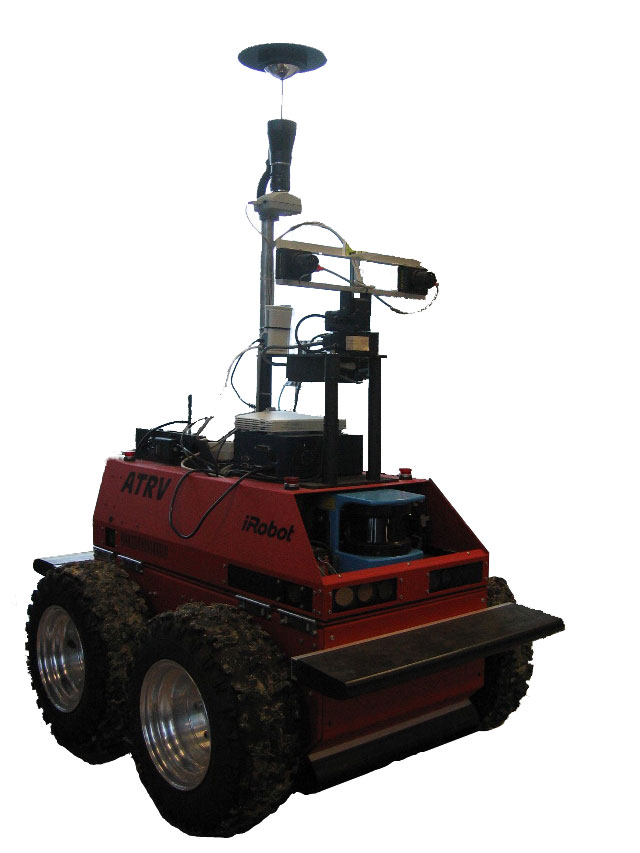
\includegraphics[width=40mm]{dala.png}}
  \caption{LAAS UGVs}
  \label{fig:ugvs}
\end{figure}

\vspace{1cm}

\section{LAAS UAVs}

There have been a number of UAV projects at LAAS: A dirigible named Karma \cite{karma}, and three fixed-wing aircraft: Lhassa \cite{lhassa}, Nirvana, and Manta. The Nirvana aircrafts were used for formation flight \cite{gautier} and not equipped with a sensing payload. Manta, a flying wing with a payload based on commodity X86 hardware, was abandoned due to it's less than convenient size and EMI issues \cite{manta}. These UAVs reuse the autopilot and ground station software and hardware from ENAC's open-source UAV system named paparazzi \cite{paparazzi}.

\section{ELROB competition}

The European Land Robot (ELROB) competition is held yearly in Belgium, and the theme alternates every year between military and civilian \cite{elrob}. For the 2011 civilian event, the competition is divided into four scenarios, namely: Reconnaissance and surveillance, Transport, Camp security, and Autonomous navigation. The primary team goal for our UAV in the competition is to assist the UGV by furnishing traversability information that will aid in the path planning process. The time to reach various waypoints is limited so locating any potential roadblocks or highly traversable terrain beyond the reaches of the UGV sensors is a potential source for route optimizations.

\chapter{Project Description}

The platform selected by the group is a low-power embedded system based on the Texas Instrument OMAP3 processor (details in Section \ref{sec:AirborneProcessor}). The Gumstix Overo module \cite{Overo}, on which the OMAP processor is mounted, provides the capacity to run the Linux operating system with minimal physical dimension and power requirements. 

The sensors selected include the Hokuyo UTM-30LX (Section \ref{Hokuyo}), a scanning laser range finder, a CMOS image sensor (Section \ref{caspa}), and an inertial navigation system (XSens MTIG, Section \ref{MTIG}). Apart from the camera, all these sensors are already used extensively at the LAAS and are supported with custom driver software developed at the LAB \cite{robotpkg}. Furthermore, these drivers have already been ported for use with the ARM processor architecture.

This payload equipment will reside on-board a low-cost R/C type of aircraft controlled by the paparazzi autopilot system as detailed in Sections \ref{sec:mentorproject} and \ref{sec:paparazzi}

\section{Airborne Processor}
\label{sec:AirborneProcessor}

\subsection{Hardware}

The central component of the payload is the Gumstix Overo board. This board contains the TI OMAP proccessor along with wifi, ethernet, bluetooth transceivers, and a convenient microSD socket. The TI OMAP System On Chip (SOC) processor incorporates a 600MHz 32-bit ARM Cortex-A8 core, a DSP, and many peripherals including UART, I2C, SPI, SD, USB, and a dedicated camera interface. The package-on-package (POP) configuration, where the SDRAM and NAND memory are stacked directly on top of the processor saves valuable space and weight and decreases EMI/EMC issues. While the camera interface and the DSP provide for future research capabilities, in the near term the important interface is USB Host as this will be used to receive laser scanner telemetry along with other serial-based communications (Intertial Navigation System and ground communication).

\subsection{Software}

The OMAP processor runs a full Linux operating system, cross compiled on a standard Linux host using a compilation system called OpenEmbedded. OE is capable of generating the necessary bootloader, linux kernel and modules, along with a root file system populated with all of the libraries and applications that might be needed to run our payload code. Configuration is done using bitbake recipes. With assistance from LAAS developers, bitbake recipes were created for the hokuyo and MTIG device libraries and are now available for the OMAP.

\section{Airborne Sensors}

\subsection{Hokuyo UTM-30LX}
\label{Hokuyo}

The UTM-30LX scans a single line around it's central axis at a rate of 40 Hz. A distance and reflectivity measurement is taken at a resolution of 1/4 of a degree, it's field of vision is 270 degrees, and distance resolution is in the millimeter range. The USB interface, along with open-source software drivers \cite{robotpkg}, allows easy interfacing with PC and embedded hosts.

\subsection{Aptina MT9V032 Camera}
\label{caspa}

The MT9V032 CMOS device from Aptina was selected due to its global shutter characteristic that guarantees that all pixels in a frame are acquired simultaneously (unlike the much more common rolling shutter cameras found in most webcams, cell phones, etc). Camera resolution is 752 x 480 pixels and is available in color or black and white. 

The CMOS Camera is interfaced to the OMAP processor using the dedicated camera bus by means of level converters (1.8V/3.3V). This direct connection is a parallel bus with a maximum clock rate of 40MHz, which allows for fast and efficient acquisition of image data. A custom designed camera board using this sensor is in the works at the LAAS while initial testing will depend on the commercially available camera board from Gumstix, INC called Caspapx \cite{caspa}.

Software support is provided as a linux driver, currently for kernel version 2.6.34. The driver has been tested to work and performance remains to be determined.

\subsection{XSens MTIG INS}
\label{MTIG}

The XSens MTIG device uses MEMS sensors along with a GPS receiver to generate attitude and position estimates at a maximum rate of 100Hz using an undocumented Kalman filter running on its embedded processor. It is optionally capable of providing raw sensor measurements at a rate up to 500Hz. The serial interface is well documented and supported with various open-source libraries including LAAS' robotpkg \cite{robotpkg}.


\section{Scan Flight Geometry}
\label{geometry}

The scanner is mounted so that the scan plane is perpendicular to the ground and the aircraft's longitudinal axis. The scan line on the ground is defined by the flight parameters as follows:

nominal UAV flight velocity : 20-30 m/s

nominal UAV flight height AGL : 30 m

Lidar sensor resolution : 1080 points over 270 deg visible (1440 points over 360 deg) @40Hz

ground covered distance during one revolution of scanner:
\begin{equation}
Dist_{per\_scan\_rev} = ground\_speed \times time_{per\_scan\_rev} = 20~\frac{m}{s} \times \frac{1}{40}~s = 0.5~m 
\end{equation}

For 90 \degree; interest zone :

scan line advances down ground track :

\begin{equation} 
Dist_{x}=  \frac{90}{360} \times Dist_{per\_scan\_rev} = \frac{1}{4} \times 0.5~m = 12.5~cm
\end{equation}

scan line proceeds along sensor rotation (for a 90 scan, this is twice the AGL height) :

\begin{equation} 
Dist_{y}=  2 \times AGL = 2 \times 30~m = 60~m
\end{equation}

Resolution :

\begin{equation}  
\frac{ \frac{90}{360} \times 1440~pixels }{scan\_length} = 
\frac{360~pixels}{\sqrt{{Dist_x}^2+{Dist_y}^2}} \approx \frac{360~pixels}{Dist_y}= 6~ \frac{pixels}{m} = 17~cm
\end{equation}

Angle relative to track : (negligible relative to crab angle)
\begin{equation} Angle_{scan\_to\_track} = \tan^{-1} \frac{Dist_x}{Dist_y} = \tan^{-1} \frac{0.125}{60} = 0.119^\circ
\end{equation}

This information is summarized in figure \ref{fig:geo1} and \ref{fig:geo2} below.

\begin{figure}[ht]
  \centering
  \subfloat[Overview]{\label{fig:geo1}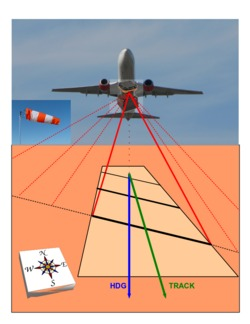
\includegraphics[width=70mm]{geo1.jpg}}                
  \subfloat[Detail]{\label{fig:geo2}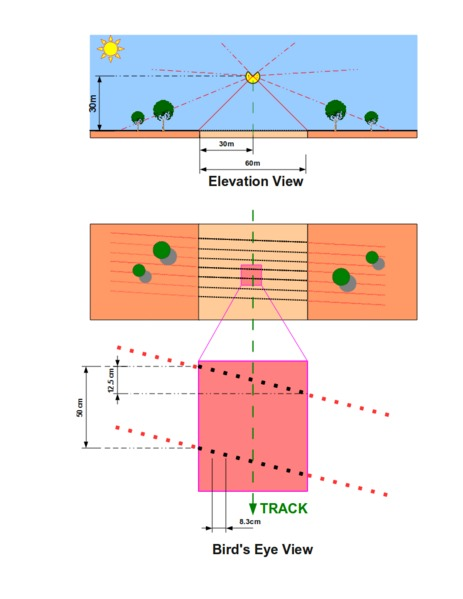
\includegraphics[width=70mm]{geo2.jpg}}
  \caption{Scan Geometry}
  \label{fig:geometry}
\end{figure}

\section{Autopilot System}
\label{sec:paparazzi}

\subsection{Paparazzi Description}

Paparazzi is an autopilot system based on a C-code mainloop program running on an airborne ARM microcontroller and Ocaml ground-station code running on a standard Linux PC or laptop \cite{paparazzi}. The system allows for extensive customization and extensions. For example, the flight plan mechanism allows the creation of complex trajectories based on waypoints and conditions. Some other options include support for multiple simultaneous aircraft and ground stations,  a software bus model that makes the creation and insertion of additional software agents into the system straightforward, and various simulation capabilities that are useful in initial testing of code and configurations. Ground to air communications are typically achieved with low-bandwidth serial modems and commercial R/C control receivers and transmitters. 

\subsection{Aircraft Types}

Paparazzi supports fixed-wing and rotating-wing aircraft. There is much recent use on quadrotor platforms, especially the Asctec airframe \cite{asctec}, but helicopter use has so far been very limited. Users of the fixed-wing configuration typically use small foam airframes such as the ones manufactured by RC manufacturer Mutliplex \cite{multiplex}, brushless electric motors, and the wingspans remain below 1.5m. In a few cases, the airframes are much larger, or much smaller, or more complex. These might incorporate fiberglass or carbon airframes for extended runtime \cite{murat} or range \cite{corsica}, or a gas turbine to achieve higher velocities, or larger wing areas and increased payload capacity. Essentially, the PID algorithms implemented in paparazzi are such that just about any standard craft can be controlled if the gains are adjusted properly.

In the most basic and most widely used fixed-wing configuration, the autopilot uses GPS and IR sensors for attitude and navigational control \cite{paparazzi_paper}. Due to some of the drawbacks of these sensors, support for replacement or complimentary sensors exists and is continuously explored. This includes the use of static and dynamic pressure sensing (to allow the aircraft to respect air-speed or altitude bounds or setpoints, for example), the use of inertial measurement units (to eliminate the need for a minimum ground/sky IR contrast, for example), and the use of a magnetometer to obtain a measure of the aircraft's heading. To maintain an accurate state estimate with small craft capable of high roll rates, the bandwidth-limited IR sensors are complemented with a roll gyro. This is typically a low-cost MEMS sensor, of the likes from Analog Devices, and interfaced via the autopilot's extra digital interfaces or sampled by an ADC channel.

\subsection{Hardware}

The current autopilot hardware is the Tiny2.1, a 50-gram board with a NXP LPC2148 microcontroller, a U-blox GPS receiver module and antenna, and small Molex Picoblade connectors for interfacing with the following devices :

\begin{itemize}
\item UART-based modem (typically Digi XBee/XBee Pro, or Aerocomm)
\item PPM-based RC receiver input (PPM signal requires receiver modification so certain users have put the effort into using serial-protocol based 2.4GHz receivers)
\item PWM-based RC servo outputs
\item USB for programming by PC Host
\item ADC inputs to sample IR sensors and monitor battery level
\item I2C and SPI interfaces for additional communication, sensor, or actuator options (see examples cited above)
\end{itemize}

\subsection{Paparazzi tradeoffs}

A typical useful hardware and software system must wrestle with the complexity trade-off. Either designs follow the KISS principle, and favor lightweight and easy to master architectures, or they aim to deliver a high degree of modularity and configurability to enable extensibility, continuous reuse and evolution. Paparazzi adopts the KISS principle for hardware designs, choosing to use COTS modules and skipping any redundancy, subscribing to the idea that a simple, straightforward, clean, and well-documented design can be relatively robust and enables a larger community (for many, a hobby activity). The software side is very different because extensibility and configurability were goals from the outset and development has continuously evolved without any milestones or official releases. This has results in a complex and sparsely documented code base that can seem unwieldy to anyone except a dedicated developer with the proper amount of pre-requisite competencies.

Like all active complex configurable systems, the challenge with paparazzi is its steep learning curve and rapid and continuous evolution. Tailoring the system for a specific application is not difficult because paparazzi requires extensive modifications, but because much of the system has to be mastered before a clear idea emerges of how and where the modifications should be made. Since documentation is limited to unstructured wiki pages and due to a complete lack in code comments, a user is essentially forced to become a developer and to dive deep into the system or resort to hacks to limit the time invested. Beyond the obvious drawbacks of the later option, is the fact that such hacks are only useful in the very short-term. Since the hacks will not be able to be merged with the software base, as the base evolves the hacks will continuously break and require constant effort to keep them working. This pressure is the reason why many users have forked the paparazzi code, added their extensive application-specific modifications without staying up to date, to end up with a system that is nearly un-mergeable with the evolved paparazzi code base. The bottom-line is that tailoring paparazzi for a project should be approached in one of two ways depending on the objectives. One, if the intent is to produce a one-off demo and future reuse is not a consideration, a fork can be considered along with quick hacks. If the continuous evolution of the application is envisioned or if sharing the capabilities with other paparazzi users is desired, the time to properly integrate customizations and continuously maintain them needs to be anticipated and allocated. This is the same sort of commitment already in place for the LAAS' openrobots software.

All this to say that considerable time is required integrate paparazzi in this project and that new team members will not able to contribute for the few months it will take to get to know the system.

\section{Challenges}

\subsection{Weight and Size}

The most convenient UAVs are those in the 1 meter wingspan range and made of foam, as these are easy to transport, repair, and pose very little security risk. But their limited payload capabilities (300 grams or less) restrict their practical uses to payloads that can be highly miniaturized. In our case, where a payload capacity of 600 grams is necessary, staying in this 1-meter regime would be possible only with the design of a custom aircraft. With the Mentor airframe, transport and repair options are still manageable, but the high-speed necessary to generate the required lift (anticipated 30+ m/s), combined with a 2.5 kg overall weight, also combined with the low altitude necessary for lidar acquisition, means that a crash is more likely due to lower reaction times and proximity to obstacles, and the increased momentum will have more grave consequences. The solution would be an airframe and wing design tailored for low-speed flight. This reduces risk and increases the density of the LIDAR-acquired point clouds. The drawback to such a design is the reduced capacity to fly in strong winds and a reduced range. The design of this aircraft would include a number of other benefits over the current craft: 

\begin{itemize}
 \item A payload bay integrated in the fuselage for reduced drag and increased protection in a crash
 \item Increase in wing area to permit slow flight
 \item Reduced wing span for easy of transport
 \item Airfoil design optimized our needs : Difficult to stall and always stays close to the designed airspeed *
\end{itemize}

(*Note: When the aircraft attempts to gain speed in a dive, the airfoil generates additional drag making the accumulation of airspeed difficult.)

Particularly in a lab setting, the major difference with the development and deployment of UAVs is that a generic kitchen sink approach is no longer possible without a large support team and an immense budget. When the research emphasis is on algorithm development, the most useful and practical research UGVs are the ones that resemble a desktop development environment (x86 PC, for example), can house a plethora or sensing and communications devices, and can be easily reconfigured. Due to these goals, UGVs are typically 5 to 100 kilograms. In the UAV context, 5 kg is already a very substantial aircraft. The conclusion is that expectations for small lab UAVs should be that each can only be good for exploring a few ideas after which it will either need to be abandoned or completely reworked. And since it's just not possible to halt an aircraft at a moments notice, crashes are more likely and it should be expected to have to rebuild periodically or build multiple aircraft up-front to avoid long reconstruction delays.

\subsection{Synchronization of Sensors}
 
Currently there is loose synchronization based on timestamps added to the scan and INS datastreams at the application level. Tighter synchronization is planned in the future by time stamping at a lower level (i.e. in the device drivers) and by hardware sync between the scanner and the camera. The pulse output generated by the scanner at the start of each revolution will be used to trigger the exposure of a camera frame using it's exposure input. This input will be available on the custom camera design currently in development at the LAAS.

\subsection{Other Challenges}

\begin{itemize}
 \item Limited LIDAR range and resolution between scan lines at high aircraft velocities.
 \item Maintaining near-constant Above-Ground-Level (AGL) altitude to stay within the 30m or less Lidar range.
 \item Detecting obstacles in the flight path to avoid tree tops, for example.
 \item Accurate attitude and position estimates needed for accurate data correction and geo-referencing.
\end{itemize}

\chapter{Ground-based Testing}

In an attempt to gain some practical experience and flesh out any limitations of the hokuyo device in an outside daylight environment, a ground-based test was carried out.

\section{Test Description}

\begin{figure}[ht]
 \centering
 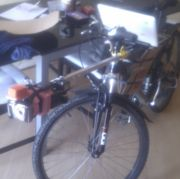
\includegraphics[width=6cm]{./Bikesciencepackage.jpg}
 % Bikesciencepackage.jpg: 180x179 pixel, 72dpi, 6.35x6.31 cm, bb=0 0 180 179
 \caption{Bike Test Vehicle}
 \label{fig:bike}
\end{figure}

The hokuyo sensor along with the MTIG was mounted on boom attached to a standard bicycle as show in Figure \ref{fig:bike}. While the bicycle traveled through a residential neighborhood a small laptop acquired the data to files. These files show that on a sunny day the hokuyo can detect at a light-colored perpendicular surface up to 20 meters away. It remains to be determined what maximum distances can be reliably detected on surfaces such as dirt and grass and at angles approaching 30 to 45 degrees from perpendicular, as will often be the case for our UAV.

\section{Output Sample}

A composite image is generated including a number of text data such as the MTIG output angles and a graphical representations of laser scan data, the location data, and video taken by a boom mounted digital camera (Figure \ref{fig:plotlogsample}). The images are then put together to create an animation showing the data along the entire path. The kokuyo data was recorded at a rate of approximately 20 Hz while the MTIG Data was near 100Hz. Rough synchronization is accomplished by using the MTIG data sample with a timestamp closest to the one in a laser scan (each laser scan is also timestamped). 

\begin{figure}[ht]
 \centering
 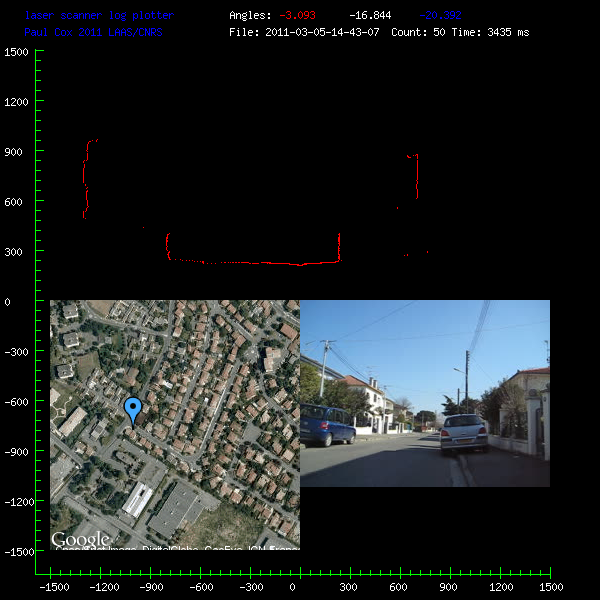
\includegraphics[width=12cm]{./Plotlogsample.png}
 \caption{Sample animation frame}
 \label{fig:plotlogsample}
\end{figure}

The test showed the hokuyo device can be used in an exterior setting and that distances of up to 16 meters can be detected even in bright sunlight if the reflecting surface is perpendicular and of a light color.

\section{Next Steps}

The next step is to represent the laser scans in a 3D environment, creating a Digital Terrain Model and representing graphically in an openGL tool such as GDHE. This process can be accomplished with the LAAS tools robotpkg and Jafar, and I am still trying to learn these so this tasks is not yet complete. To become accustomed to these tools and understand the methods behind them, I've developed various applications to work through data acquisition, generation, and processing. The code is available freely online \cite{laserhawkgit}. Some screenshots of these applications are shown below in Figure \ref{fig:mkvirt} and \ref{fig:hoku2gdhe}.

\begin{figure}[ht]
 \centering
 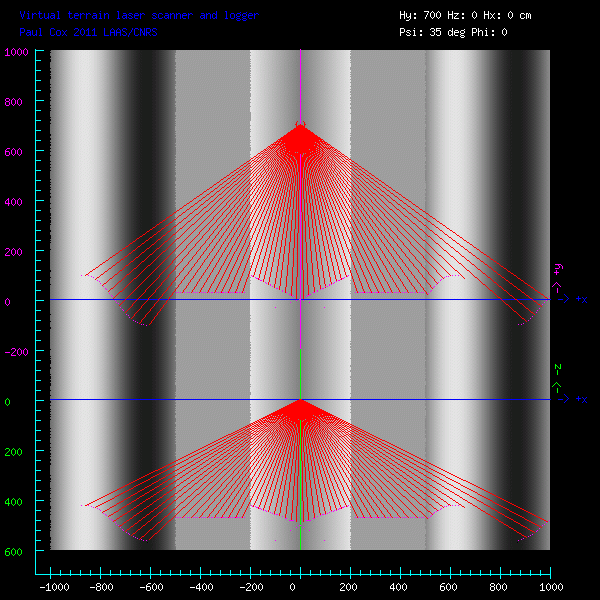
\includegraphics[width=12cm]{./Mkvirtsample.png}
 % Mkvirtsample.png: 0x0 pixel, 300dpi, 0.00x0.00 cm, bb=
 \caption{Virtual terrain simulator}
 \label{fig:mkvirt}
\end{figure}

\begin{figure}[ht]
 \centering
 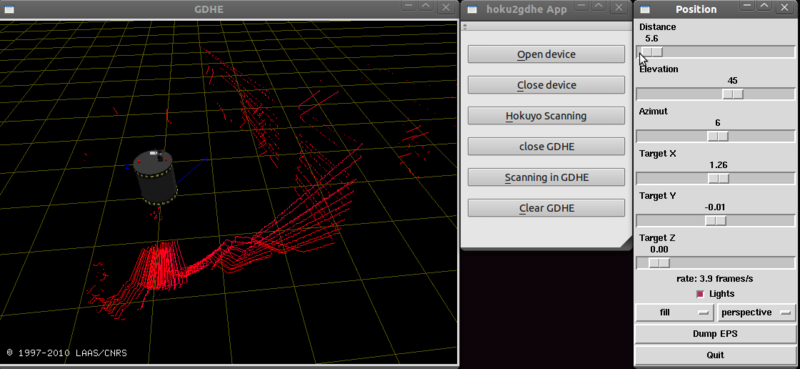
\includegraphics[width=12cm]{./Hoku2gdhe.png}
 % Hoku2gdhe.png: 0x0 pixel, 300dpi, 0.00x0.00 cm, bb=
 \caption{Data visualisation in GDHE}
 \label{fig:hoku2gdhe}
\end{figure}


\chapter{Mentor Aircraft Project}
\label{sec:mentorproject}

As explained above, the immediate goal is to outfit a Multiplex Mentor aircraft with a Hokuyo, Gumstix Overo, and MTIG for the June 2011 competition. Towards this goal, I've integrated a paparazzi autopilot in a standard Mentor airframe. I've also built a reinforced modular payload pod to hold the science package in an easy removable format. This permits development with the science package in a lab environment without being encumbered by the airplane, and provides some level of protection in the event of a crash.

\section{Airframe}

The aircraft is a standard three-axis electric R/C model and is displayed in Figure \ref{fig:mentor}. It uses two ailerons, an elevator, and a rudder for control surfaces along with a 40A speed controller for thrust control.

\begin{figure}[ht]
 \centering
 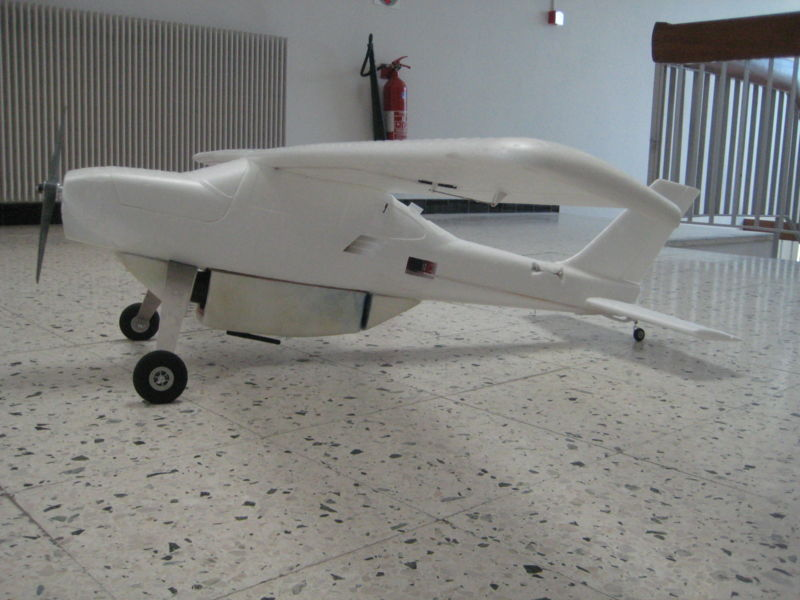
\includegraphics[width=10cm]{./800px-Mentor1_2.jpg}
 % 800px-Mentor1_2.jpg: 800x600 pixel, 180dpi, 11.29x8.47 cm, bb=0 0 320 240
 \caption{Completed Mentor Aircraft with Payload}
 \label{fig:mentor}
\end{figure}

\section{Payload}

The pod is built using typical model construction techniques. As seen in Figure \ref{fig:payload}, a plywood frame houses the various components and a glass-fiber reinforced foam cover provides a streamlined shape and protects the pod contents in the event of a crash. The payload weight is 650 grams and will require the Mentor to fly at high speed to generate the necessary lift.

\begin{figure}[ht]
 \centering
 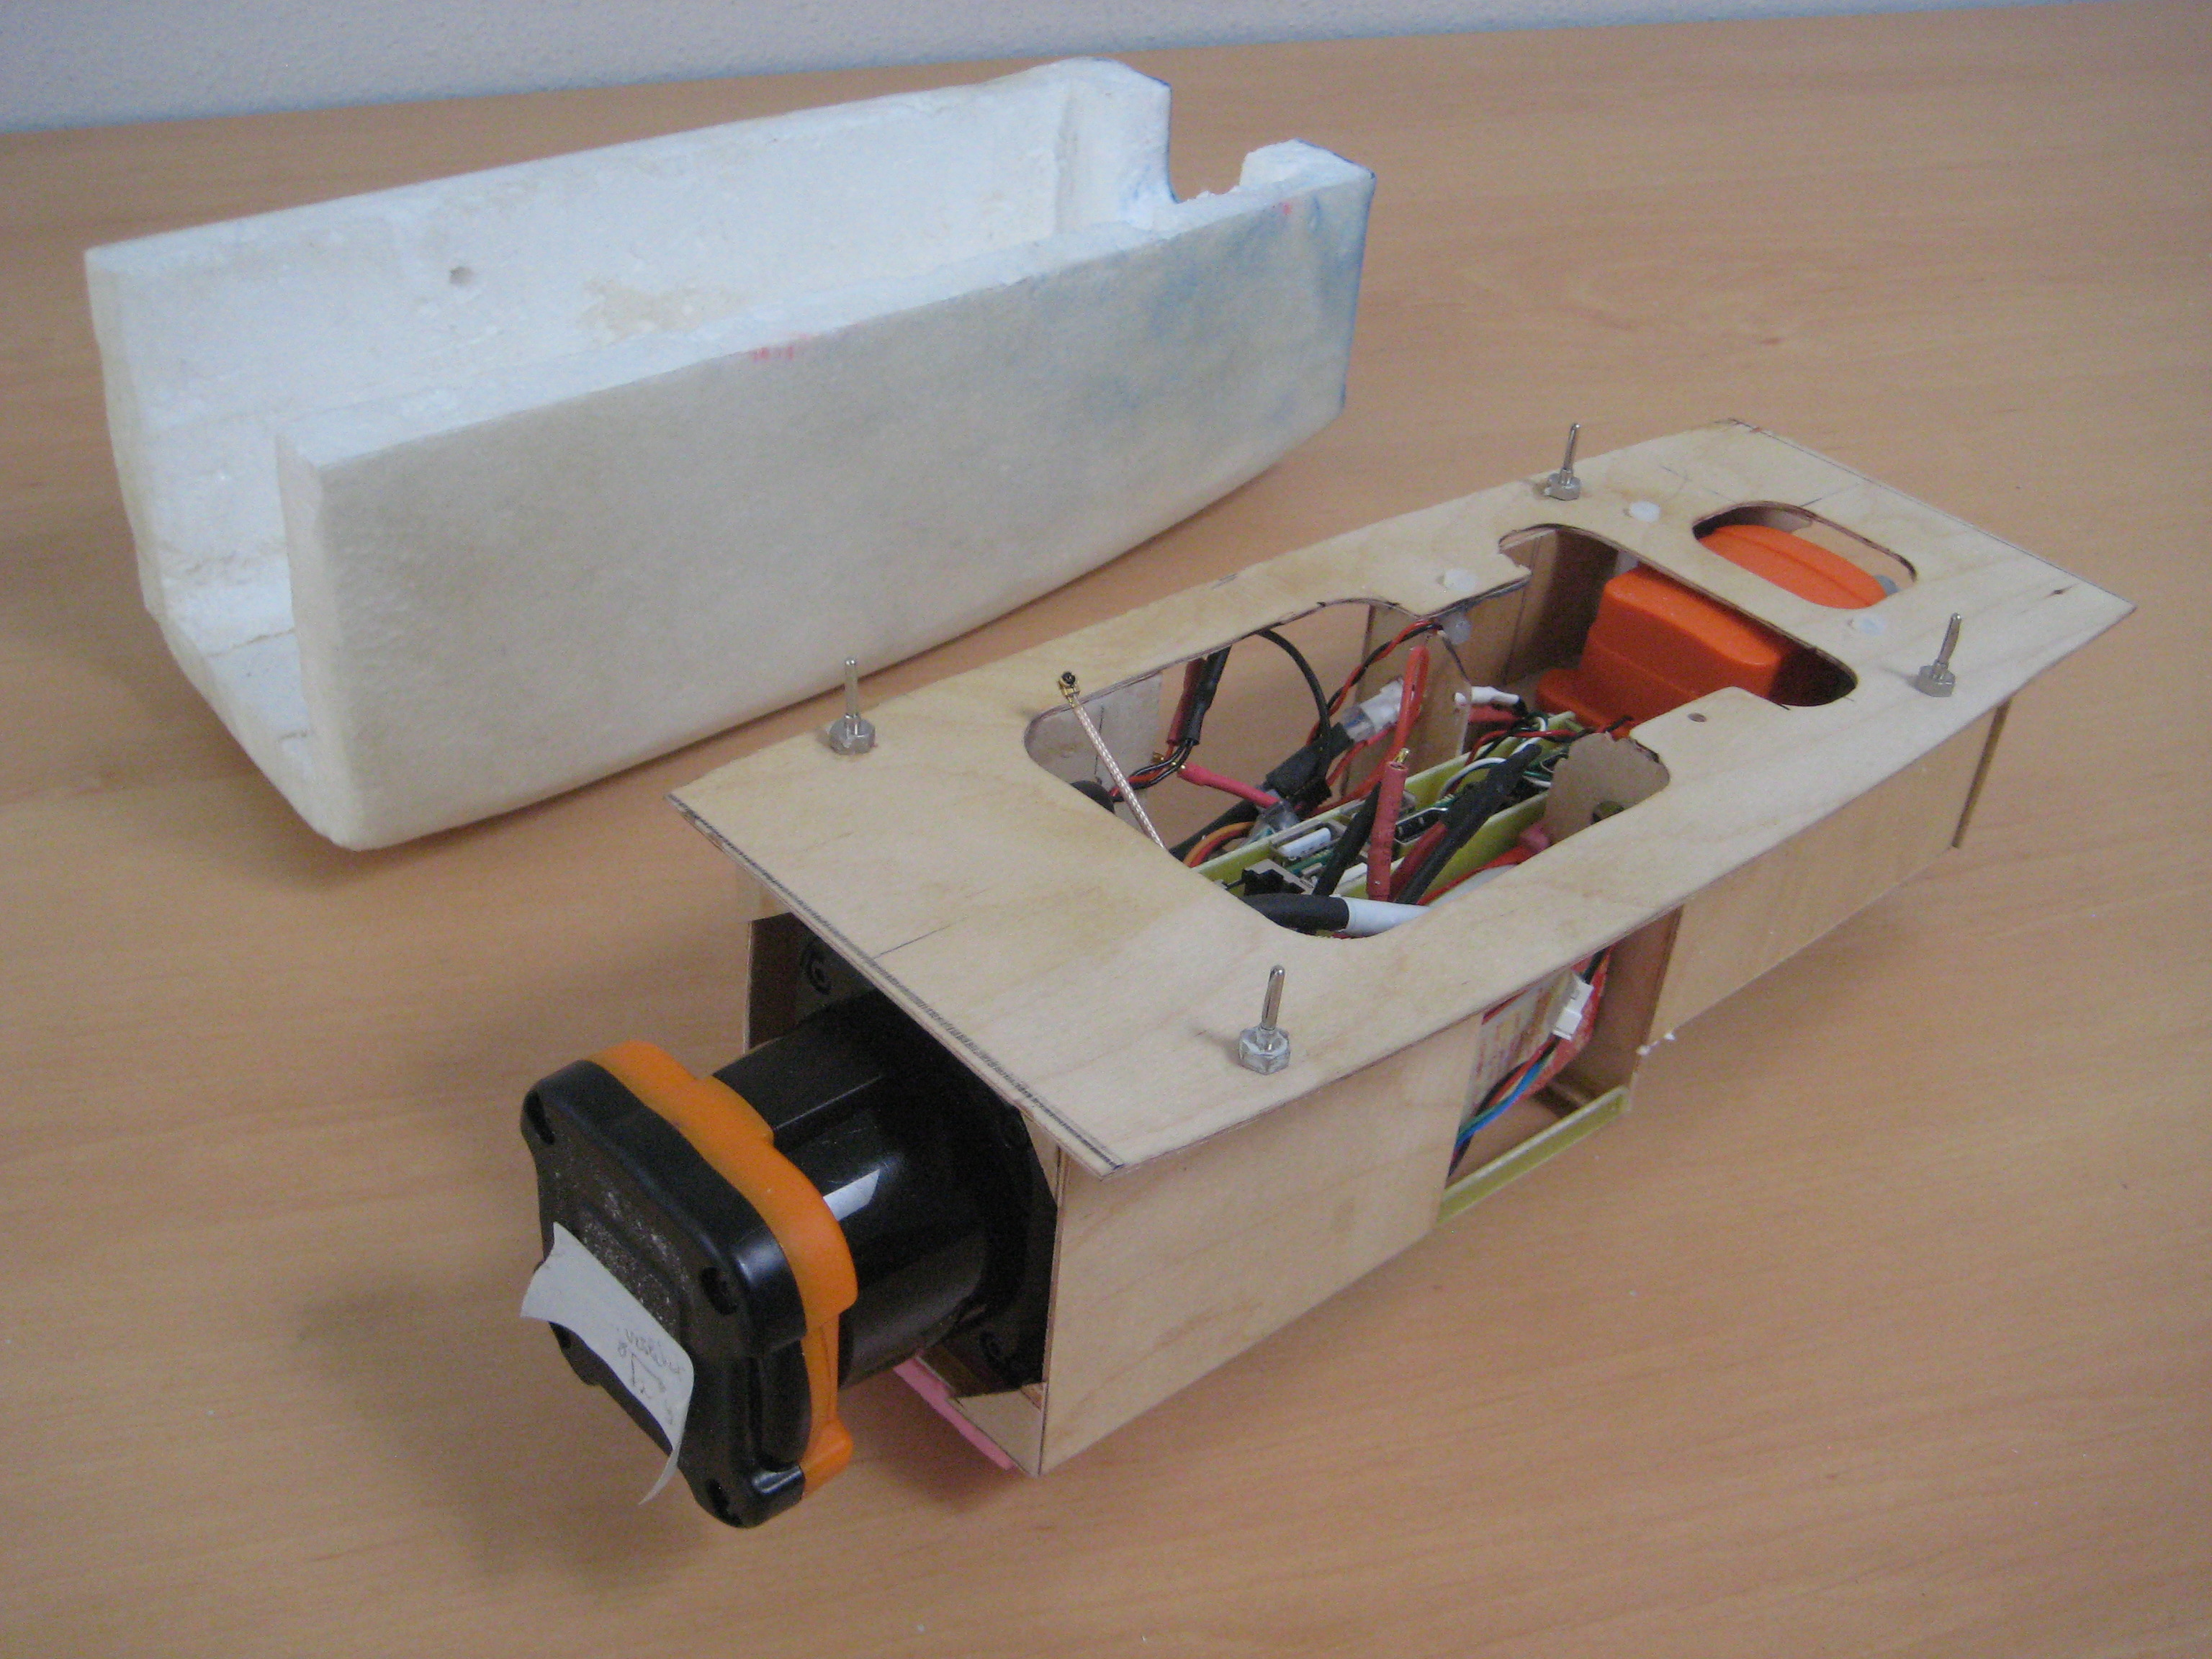
\includegraphics[width=10cm]{./Mentor1_payload2.jpg}
 % Mentor1_payload2.jpg: 3072x2304 pixel, 180dpi, 43.35x32.51 cm, bb=0 0 1229 922
 \caption{Completed Payload Pod}
 \label{fig:payload}
\end{figure}

\section{Block Diagram}

The payload electronics hardware is connected according to Figure \ref{fig:hwdiagram} below.

\begin{figure}[ht]
 \centering
 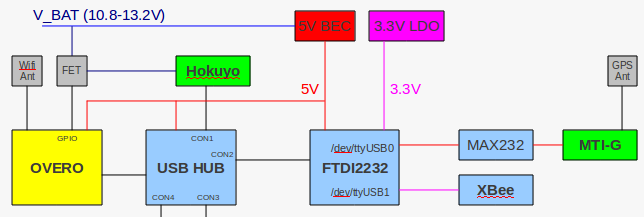
\includegraphics[width=10cm]{./payload_hardware_block_diagram.png}
 % Payload_hw_block_diagram.png: 0x0 pixel, 300dpi, 0.00x0.00 cm, bb=
 \caption{Payload Hardware Block Diagram}
 \label{fig:hwdiagram}
\end{figure}

\section{Weights}

The weight of the individual components are listed in Figure \ref{fig:weight1} and \ref{fig:weight2}.

\begin{figure}[ht]
  \centering
  \subfloat[Payload]{\label{fig:weight1}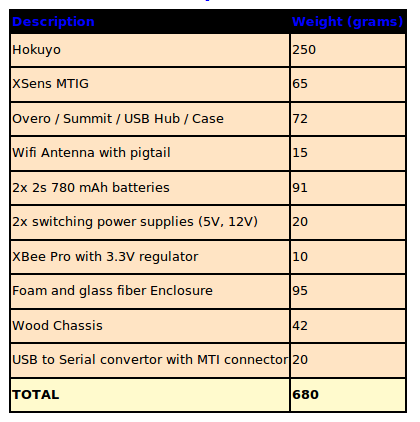
\includegraphics[width=70mm]{./weights.png}}                
  \subfloat[Overall]{\label{fig:weight2}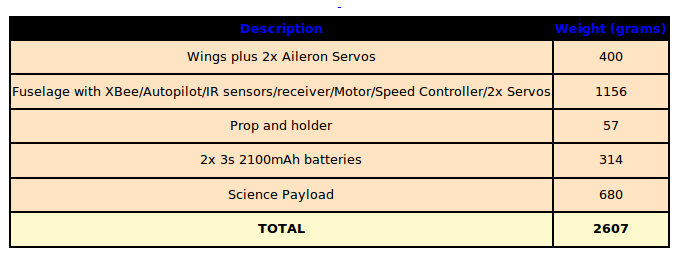
\includegraphics[width=70mm]{./weights_overall.png}}
  \caption{Weights}
  \label{fig:weights}
\end{figure} 

\chapter{Research Perspectives}

For the time being, focus is on the practical realization of a useful data set and the research aspect is limited to asking general questions about potential goals and techniques. This section is simply a collection of notes that will be developed for the final report.

Much research literature on applications of airborne lidars : very common in forestry, land management, archeology.

Techniques to reconstruct ground level by filtering obstructions, or to model buildings or land parcels, determine tree heights or diameters, estimate shore lines.

Much research uses complimentary nature of vision with lidar. 

visual servoing

\section{Traversability Mapping and DTM}

Constructing DTM, determining traversability from DTM, types of traversability maps... Obstacle detection using aerial Lidar and/or vision. Does the use of topographic maps known a-priori change the nature of the problem? How about hi-res satellite imagery? Since potential paths can be determined from these maps, UAV tasks could be to vet those paths in the goal of a classification of route options by risk, distance, time. Is completely autonomous traversability assessment a hard requirement? Wouldn't a man-in-the-loop scenario, where a supervisor be more realistic? At Elrob, human interaction is permitted but the amount of time used is proportional to the score penalty. Presenting an image mosaic, along with satellite imagery, where the potential routes are highlighted along with traversability issues along them to a human supervisor. 

UAV/UGV scenarios :
Scout : The UAV leads the UGV along the current route, scanning along given waypoints to confirm the route as traversable. 

\section{UGV UAV cooperation}

By default, UAV scans in areas complimentary to the area under acquisition by UGV. An area beyond and slightly overlapping with the UGV field of vision may be ideal. Need to determine in what scenarios UGVs would request specific areas to be scanned. For example, if robot is at a split in a path, request to UAV to map both paths. Is strategy that UGV provides goal waypoint and UAV maps area between that waypoint and the UGVs present position?

 Since the data volume is large, determining what info needs to be processed onboard and what is transmitted on ground is crucial. The tradeoff is that compute power on ground is easy but getting the data to the ground is not. Processing with simplified algorithms risks filtering useful information so a very specific goal needs to be defined and enough analysis performed to determine that . Also transmission techniques with lossy links is also a large field of study in and of itself. 

\begin{thebibliography}{9}

\bibitem{ugvs}
  \url{http://homepages.laas.fr/matthieu/robots/}

%http://spiderman-2.laas.fr/robots/index.php

\bibitem{rackham}
  \url{http://homepages.laas.fr/sara/robots/rackham/index.php}

\bibitem{jido}
  \url{http://homepages.laas.fr/matthieu/robots/jido.shtml}

\bibitem{dala}
  \url{http://homepages.laas.fr/sara/robots/dala/index.php}

\bibitem{this}
  \url{http://paparazzi.enac.fr/wiki/Laserhawk}

\bibitem{karma}
  \url{http://homepages.laas.fr/matthieu/robots/karma.shtml}

\bibitem{lhassa}
  \url{http://homepages.laas.fr/sara/robots/lhassa/index.php}

\bibitem{gautier}
  Gautier Hattenberger,
  \emph{Formation flight: evaluation of autonomous configuration control algorithms}.
  \url{homepages.laas.fr/simon/publis/HATTENBERGER-IAV-2007.pdf}
  Intelligent Robots and Systems, 2007. IROS 2007. IEEE/RSJ International Conference, 
  2007.

\bibitem{manta}
  \url{http://homepages.laas.fr/bvandepo/wiki/doku.php?id=descriptionmanta}

\bibitem{caspa}
  \url{http://wiki.gumstix.org/index.php?title=Caspa_camera_boards}

\bibitem{robotpkg}
  \url{http://www.openrobots.org/wiki}

\bibitem{laserhawkgit}
  \url{https://github.com/paulcox/laserhawk}

\bibitem{paparazzi}
  \url{http://paparazzi.enac.fr/wiki/Main_Page}

\bibitem{elrob}
  \url{http://www.elrob.org/}

\bibitem{omap}
  \url{processors.wiki.ti.com/index.php/OMAP3_Overview}

\bibitem{Overo}
  \url{http://www.gumstix.com/store/catalog/product_info.php?products_id=211}

\bibitem{asctec}
  \url{http://www.asctec.de/home-en}

\bibitem{multiplex}
  \url{http://www.multiplexusa.com/}

\bibitem{murat}
  Murat Bronz, Jean Marc Moschetta, Pascal Brisset, Michel Gorraz
  \emph{Towards a Long Endurance MAV}
  \url{http://www.recherche.enac.fr/LOTA/lib/exe/fetch.php?id=pascal_brisset&cache=cache&media=03-bronz_moschetta_ijmav.pdf}
  \url{www.emav09.org/EMAV-final-papers/paper_78.pdf}
  International Journal of Micro Air Vehicles
  Volume 1 · Number 4 · December 2009

\bibitem{corsica}
  \url{http://paparazzi.enac.fr/wiki/Corsica}

\bibitem{paparazzi_paper}
  Pascal Brisset, Antoine Drouin, Michel Gorraz, Pierre-Selim Huard and Jeremy Tyler
  \emph{The Paparazzi Solution}
  \url{http://www.recherche.enac.fr/paparazzi/papers_2006/mav06_paparazzi.pdf}
  MAV '06,
  October 2006

Juchler, Norman, Homography-based Method To Generate A Traversability Map Using Aerial Images, LAAS-CNRS Master Thesis, April 27, 2009

E. Andersen and C. Taylor. An automatic system for creating geo-referenced mosaics from mav video.  IEEE/RSJ International Conference on Intelligent Robots and Systems, 2008. IROS 2008, pages 1248-1253, 2008.

F. C. Benitez. Homography based Techniques for Unmanned Aerial Vehicle Self-Localization using Monocular Imagery. PHD thesis, 2007.

S. Bosch. Contribution a la modelisation d'environments par vision monoculaire dans un contexte de robotique aero-terrestre. PhD Thesis, 2007.

Bosch, Sebastien, Lacroix, Simon and Caballero, Fernando. Autonomous Detection of Safe Landing Areas for a UAV from Monocular Images. 2006

E. Malis, F. Chaumette, and S. Boudet. 2-1/2-d visual servoing. IEEE Transactions On Robotics And Automation, 15(2):238-250, 1999.

E. Malis and E. Marchand. Experiments with robust estimation techniques in real-time robot vision. Technical report, 2006.

E. Malis and M. Vargas. Deeper understanding of the homography decomposition for vision-based control. Technical Report 6303, INRIA, September 2007.

N. Vandapel, R. R. Donamukkala, and M. Heber. Quality assessment of traversability maps from aerial lidar data for an unmanned ground vehicle. IEEE Int'l Conf Robots and Systems IROS 2003, pages 305-310, October 2003.

\end{thebibliography}

\end{document}          
